\section{サポートベクターマシン(SVM)}
SVMは1995年にCortesらによって提案された機械学習アルゴリズムである\cite{svm}.
SVMは教師あり学習を用いる2値分類器であるが,多クラスへの拡張も可能である.
SVMは,訓練サンプル集合からデータを分類する識別関数を学習する.
この学習過程において,SVMは訓練データの中で識別関数に近いデータであるサポートベクターを得る.
そして,サポートベクターと識別関数との距離,すなわちマージンを最大化するように識別関数を構築する.
これにより,SVMは新しいデータを分類する際,
最大限のマージンを持ってデータを分類できるようになり,
未知のデータに対しても誤分類のリスクを最小限に抑えることができる.
\subsection{ハードマージンSVM}
$n$個の$N$次元教師データ$\boldsymbol{x}_i(i=1,...,n)$,
がクラス$K_1$,$K_2$の2値分類データであるとして,
対応するクラスラベルをクラス$K_1$の時に$y_i= 1$,
クラス$K_2$の時に$y_i= -1$とすると,データが線形分離可能であれば
識別関数は(\ref{decision})式のように定義される.
 $\boldsymbol{w}$は$m$次元ベクトル,$b$は識別関数のパラメータである.
\begin{align}
    \label{decision}
f(\boldsymbol{x}) = \boldsymbol{w}^T \boldsymbol{x} + b
\end{align}
すべての教師データ$\boldsymbol{x}_i(i=1,...,n)$について(\ref{learn})式の条件を満たすように
$\boldsymbol{w}$, $b$を調節する事がSVMの学習フェーズとなる.
\begin{align}
    \label{learn}
    f(\boldsymbol{x}) = \boldsymbol{w}^T \boldsymbol{x}_i + b =
    \begin{cases}
        \geq 1&  \boldsymbol{x}_i \in K_1 \\
        \leq  -1& \boldsymbol{x}_i \in K_2
    \end{cases}
\end{align}
このとき,(\ref{learn})式は(\ref{equal})式と等価になる.
\begin{align}
    \label{equal}
    y_i(\boldsymbol{w}^T \boldsymbol{x}_i + b) \geq 1
\end{align}
\begin{figure}
    \centering
    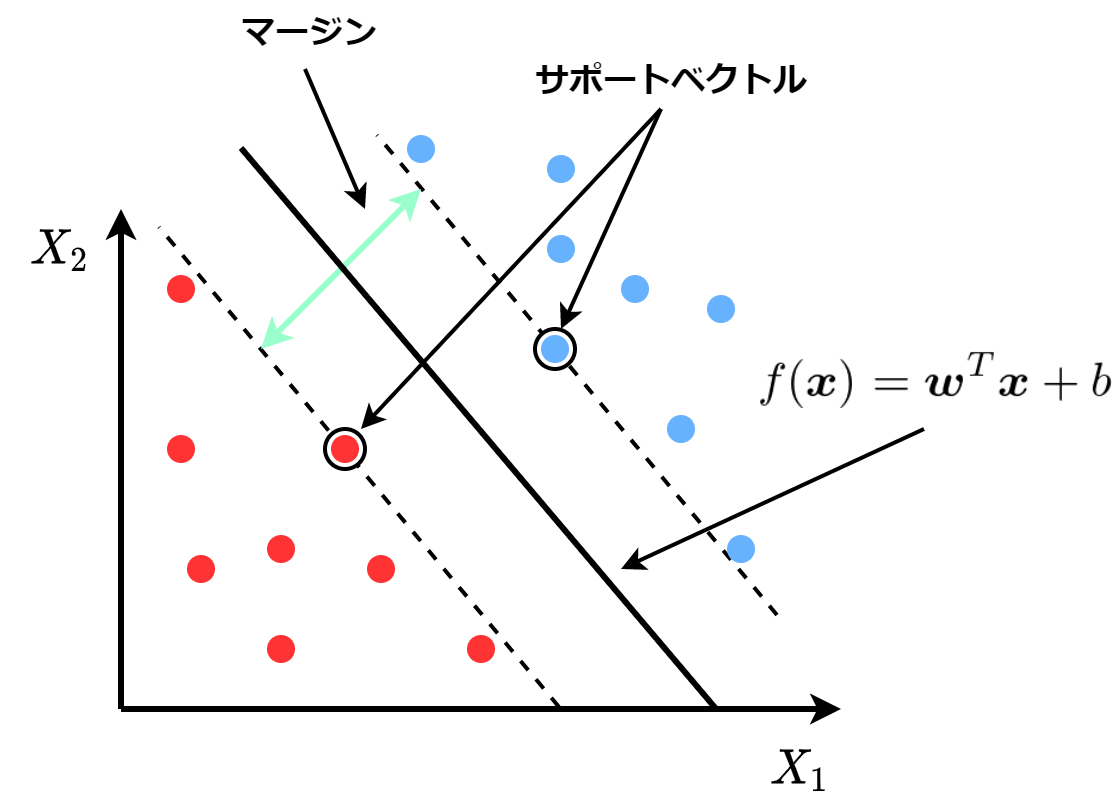
\includegraphics[width=0.6\linewidth]{svm_support.png}
    \caption{SVMの分類方法}
    \label{svm_support}
\end{figure}
ここで図~\ref{svm_support}にデータを分離する超平面(2次元では直線)を示す.
分離超平面とそれに最も近いデータ(サポートベクター)との距離をマージンと呼び,
SVMはマージンを最大化するように分離超平面を求める.
マージンを最大化することで,
サポートベクターから少しずれたデータが存在しても分類可能になり,
モデルの汎化性能が向上する.
次に,マージンを最大化する超平面を求める方法を導く.
$\boldsymbol{x}_i$から超平面への距離を$d$とすると,
$d$は(\ref{distance})式のようになる.
\begin{align}
    \label{distance}
d = \dfrac{|f(\boldsymbol{x_i})|}{\|\boldsymbol{w}\| }
\end{align}
よって,マージンを$M$とすると,
マージン最大化は(\ref{margin})式の最適化問題によって表現できる.
\begin{align}
    \label{margin}
    \underset{{\boldsymbol{w},b}}{\text{max}}~M,~~ \text{subject to } \dfrac{y_i(\boldsymbol{w}^T \boldsymbol{x}_i + b)}{\|\boldsymbol{w}\|}
    \geq M ~~  (i=1,...,n)
\end{align}
さらに,(\ref{margin})式の制約条件部分を$M$で割り,
$\frac{\boldsymbol{w}}{M\|\boldsymbol{w}\|}$と
$\frac{b}{M\|\boldsymbol{w}\|}$
をそれぞれ$\tilde{w}$,$\tilde{b}$
とすると制約条件は(\ref{chmargin})式に書き換えられる.
\begin{align}
    \label{chmargin}
    y_i(\boldsymbol{\tilde{w}}^T \boldsymbol{x}_i + \tilde{b}) \geq 1
\end{align}
(\ref{chmargin})式の等号が成立するデータ
$\boldsymbol{x_i}$は分離超平面と距離が最も近いデータ,
すなわちサポートベクターである.
したがってマージン$\tilde{M}$は(\ref{newmargin})式のようになる.
\begin{align}
    \label{newmargin}
   \tilde{M} = \dfrac{1}{\|\boldsymbol{\tilde{w}}\|}
\end{align}
よって(\ref{margin})式は(\ref{finalmargin})式で表すことができる.
\begin{align}
    \label{finalmargin}
    \underset{\boldsymbol{\tilde{w}},\tilde{b}}{\text{max}}~\dfrac{1}{\|\boldsymbol{\tilde{w}}\|},
  ~~ \text{subject to } y_i(\boldsymbol{\tilde{w}}^T \boldsymbol{x}_i + \tilde{b}) \geq 1~~  (i=1,...,n)
\end{align}
$\|\boldsymbol{\tilde{w}}\|$は正であるため,
$\frac{1}{\|\boldsymbol{\tilde{w}}\|}$を最大化する問題は,
${\|\boldsymbol{\tilde{w}}\|}^2$を最小化する問題に等しい.
$\boldsymbol{\tilde{w}}$,$\tilde{b}$を改めて$\boldsymbol{w}$,$b$と表記すると
(\ref{finalmargin})式は(\ref{minmargin})式に書き換えられ,
マージン最大化は(\ref{minmargin})式を解く問題に帰着できる.
\begin{align}
    \label{minmargin}
    \underset{\boldsymbol{w},b}{\text{min}}~\dfrac{1}{2}{\|\boldsymbol{{w}}\|}^2,
  ~~ \text{subject to } y_i(\boldsymbol{w}^T \boldsymbol{x}_i + b) \geq 1~~  (i=1,...,n)
\end{align}
さらに,制約付き最適化問題である(\ref{minmargin})式を
ラグランジュの未定乗数法により,双対問題に置き換える.
ラグランジュ乗数$\boldsymbol{\alpha} = (\alpha_1,...,\alpha_n)^T$を用いて
ラグランジュ関数$L$を(\ref{lag})式と定義する.
\begin{align}
    \label{lag}
    L(\boldsymbol{w},b,\boldsymbol{\alpha}) 
    = \dfrac{1}{2}{\|\boldsymbol{{w}}\|}^2
    - \sum_{n = 1}^{n} \alpha_i \{y_i(\boldsymbol{w}^T \boldsymbol{x}_i + b)-1\}
\end{align}
制約条件が不等式であるため,$\boldsymbol{w}$の最適解のおいて以下のKKT条件が適用できる.
\begin{subequations}
\begin{align}
   \frac{\partial L(\boldsymbol{w},b,\boldsymbol{\alpha})}{\partial \boldsymbol{w}} = 0\label{w}\\
    \frac{\partial L(\boldsymbol{w},b,\boldsymbol{\alpha})}{\partial \boldsymbol{b}} = 0\label{b}\\
    y_i(\boldsymbol{w}^T \boldsymbol{x}_i + b)-1 = 0\label{Support}\\
    \alpha_i \geq 0
\end{align}
\end{subequations}
(\ref{Support})式より,$\alpha_i = 0$または$\alpha_i > 0$で$y_i(\boldsymbol{w}^T \boldsymbol{x}_i + b)=1$
が満たされなければならない.ここで,$\alpha_i > 0$となる$\boldsymbol{x_i}$をサポートベクターと呼ぶ.
SVMは,教師データ中から,サポートベクターのみを用いて識別関数を構成する.
 (\ref{w})式, (\ref{b})式を計算すると,それぞれ(\ref{w2})式, (\ref{b2})式になる.
 \begin{subequations}
 \begin{align}
   \boldsymbol{w} = \sum_{i=1}^{n}\alpha_i y_i \boldsymbol{w_i} \label{w2}\\
   \sum_{i=1}^{n}\alpha_i y_i = 0 \label{b2}
 \end{align}
\end{subequations}
(\ref{w2})式, (\ref{b2})式を(\ref{lag})式に代入すると,
(\ref{hard1}),(\ref{hard2})式の,$\boldsymbol{\alpha}$のみで表されるハードマージンの双対問題が得られる.
これは線形分離可能な場合のみに適用でき,誤分類を許容しない.
\begin{subequations}
\begin{align}
    \underset{\boldsymbol{a}}{\text{max}} \left\{\tilde{L}(\boldsymbol{\alpha}) 
    = \sum_{i=1}^{n}\alpha_i - \dfrac{1}{2}\sum_{i,j=1}^{n}\label{hard1}
    \alpha_i\alpha_j y_i y_j \boldsymbol{x_i}^T \boldsymbol{x_j}\right\}  \\
    \text{subject to} \sum_{i=1}^{n}\alpha_i y_i = 0, \alpha_i \geq 0,\ (i=1,...,n)\label{hard2}
\end{align}
\end{subequations}
ここで,サポートベクターに対応する添字の集合をSとすると,(\ref{w2})式より,
識別関数は(\ref{s.decision})式になる.
\begin{align}
    \label{s.decision}
    D(\boldsymbol{x}) = \sum_{i\in S}a_iy_i\boldsymbol{x_i}^T\boldsymbol{x} + b
\end{align}
また,(\ref{Support})式より,$b$は(\ref{finalb})式になる.
\begin{align}
  \label{finalb}
  b =y_i - \boldsymbol{x_i}^T\boldsymbol{x}(i \in S)
\end{align}
(\ref{s.decision}),(\ref{finalb})より得られた識別関数により,
$\boldsymbol{x}$は$D(\boldsymbol{x}) > 0$ならクラス$K_1$に,
$D(\boldsymbol{x}) < 0$ならクラス$K_2$に分類する.

\subsection{ソフトマージンSVM}
2.1節で述べたハードマージンSVMは線形分離可能なことを前提としているが,現実の問題はノイズを含むデータ
などの非線形な問題が多い.
そこで非線形な問題に対しても適応できるように,(\ref{equal})式に非負の変数$\xi_i(\geq 0)$を導入する.
その式を(\ref{soft})式に示す.
\begin{align}
    \label{soft}
    y_i(\boldsymbol{w}^T \boldsymbol{x}_i + b) \geq 1 - \xi_i
\end{align}
これにより,マージンの内側にデータが存在することを許容する.
このときソフトマージンの最適化問題は,(\ref{soft1})式,(\ref{soft2})式になる.
ここで$C$は誤分類をどれだけ許容するかを決めるハイパーパラメータであり,
小さいほど誤分類を許容し,大きいほど誤分類を許容しない.よって
この問題は,(\ref{soft1})式の第1項のマージン最大化と
第2項の誤分類の許容数のバランスを図る問題である.
\begin{subequations}
\begin{align}
    \underset{\boldsymbol{w},b,\boldsymbol{\xi}}{\text{min}}~\dfrac{1}{2}{\|\boldsymbol{{w}}\|}^2
    &+C\sum_{i=1}^{n}\xi_i \label{soft1}\\
   \text{subject to } y_i(\boldsymbol{w}^T \boldsymbol{x}_i + b) \geq &1 - \xi_i,\xi_i \geq 0 ~(i=1,...,n)\label{soft2}
\end{align}
\end{subequations}
2.1節と同様に,(\ref{soft1})式,(\ref{soft2})式を主問題として,ラグランジュの未定乗数法により双対問題を導出する.
ラグランジュ乗数$\boldsymbol{\alpha} = (\alpha_1,...,\alpha_n)^T$,
$\boldsymbol{\beta} = (\beta_1,...,\beta_n)^T$を用いて
ラグランジュ関数$L$を(\ref{slag})式と定義する.
\begin{align}
    \label{slag}
    L(\boldsymbol{w},b,\boldsymbol{\xi},\boldsymbol{\alpha},\boldsymbol{\beta}) 
    = \dfrac{1}{2}{\|\boldsymbol{{w}}\|}^2+C\sum_{i=1}^{n}\xi_i
    - \sum_{n = 1}^{n} \alpha_i \{y_i(\boldsymbol{w}^T \boldsymbol{x}_i + b)-1+\xi_i\}
    -\sum_{i=1}^{n}\beta_i\xi_i
\end{align}
制約条件が不等式であるため,$\boldsymbol{w}$の最適解のおいて以下のKKT条件が適用できる.
\begin{subequations}
\begin{align}
   \frac{\partial L(\boldsymbol{w},b,\boldsymbol{\xi},\boldsymbol{\alpha},\boldsymbol{\beta})}{\partial \boldsymbol{w}} = 0\label{sw}\\
    \frac{\partial L(\boldsymbol{w},b,\boldsymbol{\xi},\boldsymbol{\alpha},\boldsymbol{\beta})}{\partial \boldsymbol{b}} = 0\label{sb}\\
    \frac{\partial L(\boldsymbol{w},b,\boldsymbol{\xi},\boldsymbol{\alpha},\boldsymbol{\beta})}{\partial \boldsymbol{\xi}} = 0\label{sxi}\\
    \alpha_i \{y_i(\boldsymbol{w}^T \boldsymbol{x}_i + b)-1+\xi_i\}=0\label{sSupport}\\
    \beta_i\xi_i = 0\label{bxi}\\
    \alpha_i \geq 0 ,\beta_i \geq 0,\xi_i \geq 0 
\end{align}
\end{subequations}
 (\ref{sw})〜(\ref{sxi})式を計算すると,それぞれ(\ref{sw2})〜(\ref{sb2})式になる.
 \begin{subequations}
 \begin{align}
   \boldsymbol{w} = \sum_{i=1}^{n}\alpha_i y_i \boldsymbol{w_i} \label{sw2}\\
   \sum_{i=1}^{n}\alpha_i y_i = 0 \\
   \alpha_i + \beta_i = C\label{sb2}
 \end{align}
\end{subequations}
(\ref{sw2})〜(\ref{sb2})式を(\ref{slag})式に代入すると,
$\boldsymbol{\alpha}$のみで表されるソフトマージンの双対問題(\ref{finalsoftmargin1}),(\ref{finalsoftmargin2})式が得られる.
\begin{subequations}
\begin{align} 
    \underset{\boldsymbol{a}}{\text{max}} \left\{\tilde{L}(\boldsymbol{\alpha}) 
    = \sum_{i=1}^{n}\alpha_i - \dfrac{1}{2}\sum_{i,j=1}^{n}\label{finalsoftmargin1}
    \alpha_i\alpha_j y_i y_j \boldsymbol{x_i}^T \boldsymbol{x_j}\right\} \\
    \text{subject to} \sum_{i=1}^{n}\alpha_i y_i = 0,0 \leq \alpha_i \leq C,\ (i=1,...,n)\label{finalsoftmargin2}
\end{align}
\end{subequations}
識別関数はハードマージンSVMと同じく(\ref{s.decision}),(\ref{finalb})式になる.
よってソフトマージンSVMとハードマージンSVMの違いは,$\alpha_i$の上限$C$の有無だけの違いである,
本研究ではハイパーパラメータである$C$を最適化対象に含める.

\subsection{カーネルトリック}
2.2節で述べたソフトマージンSVMによって,非線形な問題に対しても分類できるようになったが, 
非線形で複雑な分類問題に対しては高性能な分類器を構成できない.    
そこでSVMは,$N$次元特徴ベクトルを$N^{\prime} $次元特徴空間に写像し,
特徴空間上で分離超平面を得る.
高次元空間への写像の例を図~\ref{syazou}に示す.
この例では,$X_1X_2$の軸を新たに追加することによって元の次元では非線形なデータを線形分離可能にしている.
\begin{figure}
    \centering
    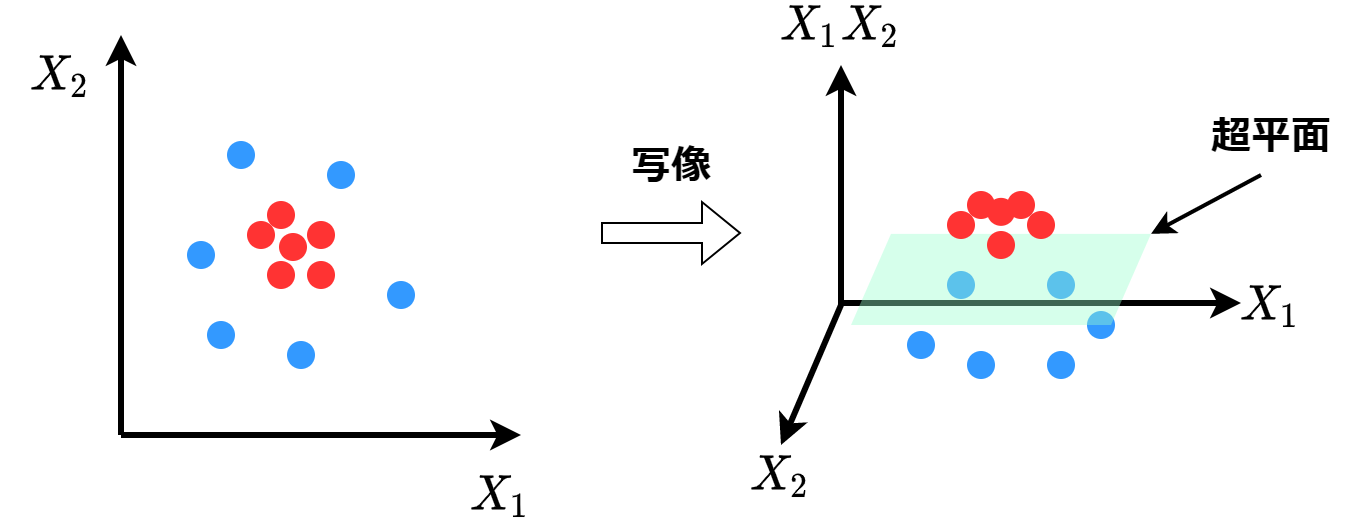
\includegraphics[width=0.8\linewidth]{syazou.png}
    \caption{高次元空間への写像の例}
    \label{syazou}
\end{figure}
一般に,線形分離可能性はデータのサンプル数が多くなればなるほど難しくなり,
特徴空間の次元数が大きくなるほど易しくなる.特に,$n-1$次元空間では,
最大で$n$個のデータを任意のラベル付けで線形分離可能である.
そのため$N$次元特徴ベクトルを$N^{\prime} $次元特徴空間に写像することで線形分離可能性が向上する.
ここで,$N$次元特徴ベクトルを$N^{\prime} $次元特徴空間に写像する関数を
$\boldsymbol{\phi}(\boldsymbol{x}) = \{\phi_i(\boldsymbol{x}),...,\phi_{N^{\prime}}(\boldsymbol{x})\}^T$
とすると,特徴空間上での分離超平面は(\ref{feature1}),(\ref{feature2})式の最適化問題を解くことで得られる.
\begin{subequations}
\begin{align}  
    \underset{\boldsymbol{a}}{\text{max}} \left\{\tilde{L}(\boldsymbol{\alpha}) 
    = \sum_{i=1}^{n}\alpha_i - \dfrac{1}{2}\sum_{i,j=1}^{n}\label{feature1}
    \alpha_i\alpha_j y_i y_j \boldsymbol{\phi}(\boldsymbol{x_i})^T \boldsymbol{\phi}(\boldsymbol{x_j})\right\}  \\
    \text{subject to} \sum_{i=1}^{n}\alpha_i y_i = 0,0 \leq \alpha_i \leq C,\ (i=1,...,n)\label{feature2}
\end{align}
\end{subequations}
しかし次元$N^{\prime}$が大きくなればなるほど
$\boldsymbol{\phi}(\boldsymbol{x_i})^T \boldsymbol{\phi}(\boldsymbol{x_j})$
の計算量が膨大になる.
そこでカーネル関数を(\ref{karnel})式で定義する.
\begin{align}
    \label{karnel}
  K( \boldsymbol{x_i}, \boldsymbol{x_j}) = \boldsymbol{\phi}(\boldsymbol{x_i})^T \boldsymbol{\phi}(\boldsymbol{x_j})
\end{align}
もし,(\ref{karnel})式を満たすようなカーネル関数が存在するならば,入力特徴ベクトルの内積計算で
$\boldsymbol{\phi}(\boldsymbol{x})$
を得ることができる.すなわち計算量が膨大になる可能性がある
$\boldsymbol{\phi}(\boldsymbol{x_i})^T \boldsymbol{\phi}(\boldsymbol{x_j})$
を直接計算する必要がない.このように内積計算をカーネル関数で置き換える手法をカーネルトリックと呼ぶ.
本実験では,(\ref{k1})〜(\ref{k4})式で表されるカーネル関数をハイパーパラメータの対象とする.
また,(\ref{k1})〜(\ref{k4})式内にあるハイパーパラメータは$\gamma$,coef0,$d$の3つである.
\begin{align}
    \text{線形カーネル:} \quad K(\boldsymbol{x_i}, \boldsymbol{x_j}) &= \boldsymbol{x_i}^T \cdot \boldsymbol{x_j}\label{k1} \\
    \text{RBFカーネル:} \quad K(\boldsymbol{x_i}, \boldsymbol{x_j}) &= \exp\left(-\gamma \| \boldsymbol{x_i} - \boldsymbol{x_j} \|^2\right)\label{k2} \\
    \text{シグモイドカーネル:} \quad K(\boldsymbol{x_i}, \boldsymbol{x_j}) &= \tanh(\gamma \boldsymbol{x_i}^T \cdot \boldsymbol{x_j} + \text{coef0}) \label{k3}\\
    \text{多項式カーネル:} \quad K(\boldsymbol{x_i}, \boldsymbol{x_j}) &= (\gamma\boldsymbol{x_i}^T \cdot \boldsymbol{x_j} + \text{coef0})^d\label{k4}
\end{align}
%カーネル関数の条件を挙げるべきか(勉強不足)
\subsection{多クラス分類への拡張}
SVMは2値分類器であるが,1対他法や1対1法により多クラス分類への拡張ができる.
1対他法では,各クラスに対し,そのクラスとそれ以外のクラスの分類をする.
そのためクラスが$K$個ある場合,$K$個のSVMモデルを用意する必要がある.
一方,1対1法では各クラスのペアの組み合わせに対して分類をする.
そのためクラスが$K$個ある場合,$\frac{K(K-1)}{2}$個のSVMモデルを用意する必要がある.
以上より,より計算量が少ないのが1対他法,より詳細な分類をするのが1対1法の特徴である.
本研究では一対他法を使用する.

